\chapter{TTL y CMOS}
%\graphicspath{ {images/} }

\section{Introducción}
El objetivo aquí fue el de implementar circuitos con compuertas lógicas de distinta tecnologías y observar la compatibilidad entre estas. 
En primer lugar se verifico el correcto funcionamientos de estas compuertas realizando las respectivas pruebas sobre las mismas por separado, estos circuitos consisten simplemente de compuertas AND de tecnología TTL y OR de tecnología CMOS obteniendo en ambos casos los resultados esperados según que compuerta era analizada.
\section{Compatibilidad}
Sin embargo al trabajar con ambos circuitos en conjunción se vio que las salidas obtenidas no se condecían con los resultados esperados, este circuito es el que se muestra a continuación:
\begin{center}
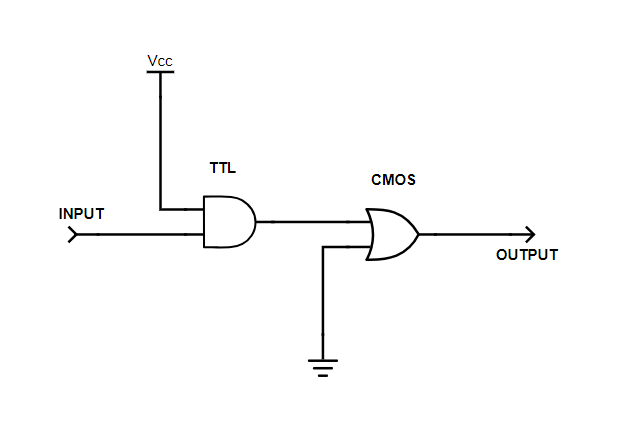
\includegraphics[scale = 0.8,keepaspectratio]{../5-TTL&CMOS/E3-ej5-defectuoso.png}
\end{center}
Se observó que al enviar una señal de entrada de 5V al circuito, es decir un 1 en términos lógicos, este entregaba una señal de salida de pocos milivolts, un 0, lo cual no es la salida esperada ya que un bit de valor 1 a la entrada del sistema genera un 1 como salida al AND el cual a su vez debiera generar un 1 a la salida de la compuerta OR.
El problema aquí es el hecho de las tecnologías con las cuales se trabaja no resultan compatibles entre si para el correcto funcionamiento del circuito. Haciendo un análisis más exhaustivo al ver los datasheets del circuito integrado 74LS08, conjunto de compuertas AND de tecnología TTL, se puede ver que este posee un \textit{HIGH-level output voltaje} típico de 3.4V mientras que por otro lado el 74HC32, circuito integrado usado para las compuertas OR de tecnología CMOS, tiene un \textit{HIGH-level input voltage} típico ligeramente mayor a 3.15V para la tensión con la cual se alimentaron los integrados. Siendo que la tensión a partir de la cual la compuerta OR interpreta un 1 es fácilmente superior a aquella que devuelve la AND para dicho bit en ningún caso la OR interpretara un 1 a su entrada, obteniendo en todo caso un bit de 0 a la salida.
\section{Solución}
El problema entonces a solucionar es el de convertir la tensión de salida \textit{HIGH} del TTL a una que pueda ser interpretable como tal a la entrada para la tecnología CMOS.
Para esto lo que se decidio implementar es lo siguiente, se considero es uso de una resistencia \textit{pull-up} junto con un transistor BJT tipo NPN para aumentar el valor de la tensión previo a entrar a la compuerta OR, sin embargo si la tensión a la base del transistor es mayor a aquella con la cual se polariza el transistor no se cumplirá la función deseada, por eso se colocó una compuerta inversora a la salida de la AND teniendo el resguardo de que ambas de estas sean de la misma tecnología. el circuito final es el que se muestra en la siguiente imagen.
\begin{center}
	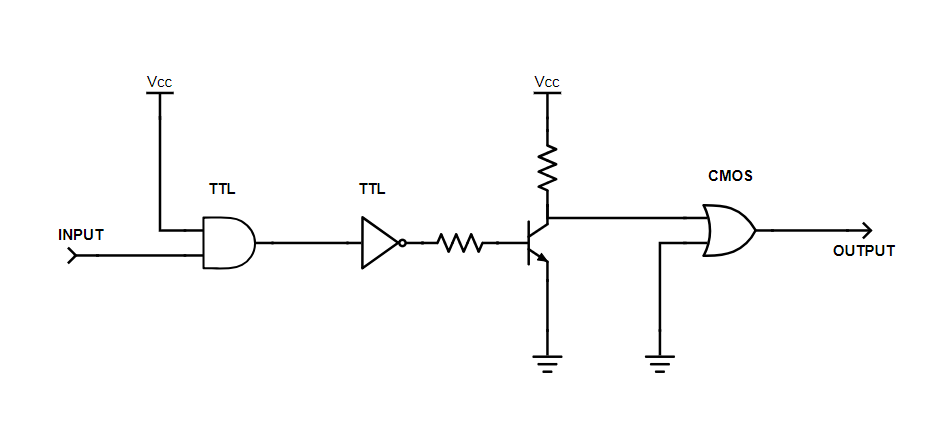
\includegraphics[scale = 0.8,keepaspectratio]{../5-TTL&CMOS/E3-ej5-corregido.png}
\end{center}

Siguiendo la lógica del circuito se entiende que cuando la compuerta AND vea un 1 a su salida el transistor no se polarizara de modo tal que la tensión a la entrada de la compuerta and será la de alimentación, siendo esta de 5v suficiente para ser tomada como 1, en la práctica se pudo ver que en este caso la compuerta AND se accionaba sin ningún tipo de problema.
Un defecto de diseño sin embargo es la disipación de potencia, perjudicial esta para el medio ambiente. Cuando en bit de input sea de valor 0 el transistor BJT estará polarizado de modo tal que habrá una constante caída de tensión sobre las resistencias.
Por último se aclara que el valor de las resistencias no fue de relevancia para el funcionamiento del circuito siendo estas de 1k, aunque un valor más elevado disiparía una menor cantidad de potencia en relación con lo anterior expuesto.
